%% Copyright (c) 2015-2019, RTE (http://www.rte-france.com)
%% See AUTHORS.txt
%% All rights reserved.
%% This Source Code Form is subject to the terms of the Mozilla Public
%% License, v. 2.0. If a copy of the MPL was not distributed with this
%% file, you can obtain one at http://mozilla.org/MPL/2.0/.
%% SPDX-License-Identifier: MPL-2.0
%%
%% This file is part of Dynawo, an hybrid C++/Modelica open source time domain simulation tool for power systems.

\documentclass[a4paper, 12pt]{report}

%% Except where otherwise noted, content in this documentation is Copyright (c)
%% 2015-2019, RTE (http://www.rte-france.com) and licensed under a
%% CC-BY-4.0 (https://creativecommons.org/licenses/by/4.0/)
%% license. All rights reserved.

% Latin Modern fam­ily of fonts
\usepackage{lmodern}

\usepackage[english]{babel}

% specify encoding
\usepackage[utf8]{inputenc} % input
\usepackage[T1]{fontenc} % output

% Document structure setup
\usepackage{titlesec} % To change chapter format
\setcounter{tocdepth}{3} % Add subsubsection in Content
\setcounter{secnumdepth}{3} % Add numbering for subsubsection
\setlength{\parindent}{0pt} % No paragraph indentation

% Change title format for chapter
\titleformat{\chapter}{\Huge\bf}{\thechapter}{20pt}{\Huge\bf}

% To add links on page number in Content and hide red rectangle on links
\usepackage[hidelinks, linktoc=all]{hyperref}
\usepackage[nottoc]{tocbibind}  % To add biblio in table of content
\usepackage{textcomp} % For single quote
\usepackage{url} % Allow linebreaks in \url command
\usepackage{listings} % To add code samples

% Default listings parameters
\lstset
{
  aboveskip={1\baselineskip}, % a bit of space above
  backgroundcolor=\color{shadecolor}, % choose the background color
  basicstyle={\ttfamily\footnotesize}, % use font and smaller size \small \footnotesize
  breakatwhitespace=true, % sets if automatic breaks should only happen at whitespace
  breaklines=true, % sets automatic line breaking
  columns=fixed, % nice spacing -> fixed / flexible
  mathescape=false, % escape to latex false
  numbers=left, % where to put the line-numbers
  numberstyle=\tiny\color{gray}, % the style that is used for the line-numbers
  showstringspaces=false, % do not emphasize spaces in strings
  tabsize=4, % number of spaces of a TAB
  texcl=false, % activates or deactivates LaTeX comment lines
  upquote=true % upright quotes
}

% Avoid numbering starting at each chapter for figures
\usepackage{chngcntr}
\counterwithout{figure}{chapter}

\usepackage{tikz} % macro pack­age for cre­at­ing graph­ics
\usepackage{pgfplots} % draws func­tion plots (based on pgf/tikz)

\usepackage{algorithm} % Add algorithms
\usepackage[noend]{algpseudocode} %  all end ... lines are omitted in algos

\usepackage{amsmath} % Add math­e­mat­i­cal fea­tures
\usepackage{schemabloc} % Add block diagram library (french one)

\usepackage{adjustbox} % Add box for flowchart

\usepackage{booktabs} % for toprule and midrule in tables

\usepackage{tabularx}

\usepackage[nolist]{acronym} % don’t write the list of acronyms.
% Acronyms list
\begin{acronym}
\acro{BDF}{Backward Differentiation Formula}
\acro{BE}{Backward Euler}
\acro{DAE}{Differential Algebraic Equations}
\acro{IDA}{Implicit Differential-Algebraic solver}
\acro{LLNL}{Lawrence Livermore National Lab}
\acro{KINSOL}{Krylov Inexact Newton SOLver}
\acro{NR}{Newton-Raphson}
\acro{PLL}{Phase-Locked Loop}
\acro{SVC}{Static Var Compensator}
\acro{SUNDIALS}{SUite of Nonlinear and DIfferential/ALgebraic equation Solvers}
\acro{WECC}{Western Electricity Coordinating Council}
\end{acronym}

% Syntax highlight
%% Except where otherwise noted, content in this documentation is Copyright (c)
%% 2015-2019, RTE (http://www.rte-france.com) and licensed under a
%% CC-BY-4.0 (https://creativecommons.org/licenses/by/4.0/)
%% license. All rights reserved.

\usepackage{color}

\definecolor{blue}{rgb}{0,0,1}
\definecolor{lightblue}{rgb}{.3,.5,1}
\definecolor{darkblue}{rgb}{0,0,.4}
\definecolor{red}{rgb}{1,0,0}
\definecolor{darkred}{rgb}{.56,0,0}
\definecolor{pink}{rgb}{.933,0,.933}
\definecolor{purple}{rgb}{0.58,0,0.82}
\definecolor{green}{rgb}{0.133,0.545,0.133}
\definecolor{darkgreen}{rgb}{0,.4,0}
\definecolor{gray}{rgb}{.3,.3,.3}
\definecolor{darkgray}{rgb}{.2,.2,.2}
\definecolor{shadecolor}{gray}{0.925}

% **********************************************************************************
% Syntax : Bash (bash)
% **********************************************************************************

\lstdefinelanguage{bash}
{
  keywordstyle=\color{blue},
  morekeywords={
    cd,
    export,
    source},
  numbers=none,
  deletekeywords={jobs}
}

% **********************************************************************************
% Syntax : XML
% **********************************************************************************

\lstdefinelanguage{XML}
{
  morestring=[s][\color{purple}]{"}{"},
  morecomment=[s][\color{green}]{<?}{?>},
  morecomment=[s][\color{green}]{<!--}{-->},
  stringstyle=\color{black},
  identifierstyle=\color{blue},
  keywordstyle=\color{red},
  morekeywords={
    xmlns,
    xsi,
    noNamespaceSchemaLocation,
    type,
    source,
    target,
    version,
    tool,
    transRef,
    roleRef,
    objective,
    eventually}
}

% **********************************************************************************
% Syntax : Modelica (modelica)
% **********************************************************************************
\lstdefinelanguage{Modelica}{
  alsoletter={...},
  morekeywords=[1]{ % types
      Boolean,
      Integer,
      Real},
  keywordstyle=[1]\color{red},
  morekeywords=[2]{ % keywords
    algorithm,
    and,
    annotation,
    assert,
    block,
    class,
    connector,
    constant,
    discrete,
    else,
    elseif,
    elsewhen,
    end,
    equation,
    exit,
    extends,
    external,
    false,
    final,
    flow,
    for,
    function,
    if,
    in,
    inner,
    input,
    import,
    loop,
    model,
    nondiscrete,
    not,
    or,
    outer,
    output,
    package,
    parameter,
    public,
    protected,
    record,
    redeclare,
    replaceable,
    return,
    size,
    terminate,
    then,
    true,
    type,
    when,
    while},
  keywordstyle=[2]\color{darkred},
  morekeywords=[3]{ % functions
    abs,
    acos,
    asin,
    atan,
    atan2,
    Complex,
    connect,
    conj,
    cos,
    cosh,
    cross,
    der,
    edge,
    exp,
    fromPolar,
    imag,
    noEvent,
    pre,
    sign,
    sin,
    sinh,
    sqrt,
    tan,
    tanh},
  keywordstyle=[3]\color{blue},
  morecomment=[l][\color{green}]{//}, % comments
  morecomment=[s][\color{green}]{/*}{*/}, % comments
  morestring=[b][\color{pink}]{'}, % strings
  morestring=[b][\color{pink}]{"}, % strings
}


\usepackage{xspace} % Define typography
\usepackage{dirtree}
\newcommand{\Dynawo}[0]{Dyna$\omega$o\xspace}


\begin{document}

\chapter{IEEE14 with proportional regulations}

The IEEE 14-bus system is a standard test case in the power system community. It represents a simple approximation of the American Electric Power system (in the U.S. Midwest) as it was in the early 1960s. The data were provided by Iraj Dabbagchi of AEP and converted into the IEEE Common Data Format by Rich Christie at the University of Washington in August 1993.

% Generic description of the non regression test
% List of scenarios
\section{Test case description}

The IEEE 14-bus test case system has 14 buses, 5 generators (three of them being synchronous compensators used only for reactive support), 1 shunt, 3 transformers, 16 lines and 11 loads.\\
There are two voltage levels in the test case: 69 kV and 13.8 kV. The lower part of the system, with generators 1, 2 and 3, corresponds to the 69 kV network, whereas the upper part is the 13.8 kV network.

\begin{figure}[H]
  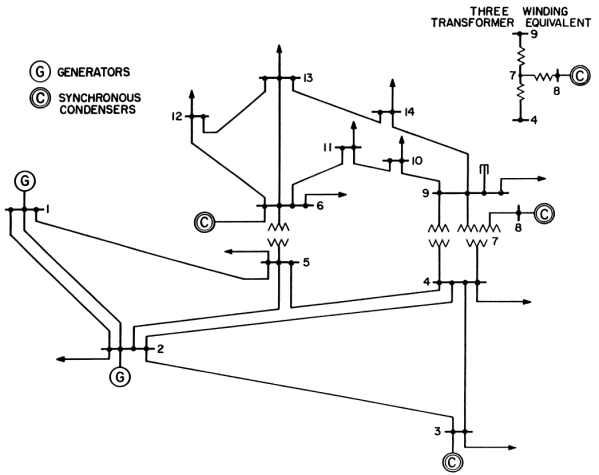
\includegraphics[width=\textwidth]{Single-line-diagram-of-IEEE-14-bus-system.png}
  \caption{IEEE 14 bus system diagram}
\end{figure}

\subsection{Initial Conditions}

The reference angle for the load flow is set at bus n°1. \\

Here are the initial conditions for each generator.

\begin{center}
\begin{tabular}{|c|c|c|c|c|}
  \hline
  Generator & P (MW) & Q (Mvar) & U (kV) & $\Theta$ (°) \\
  \hline
  1 & 232.39 & -16.55 & 73.14 & 0.00\\
  2 & 40.00 & 43.56 & 72.11 & -4.98\\
  3 & 0.00 & 25.07 & 69.69 & -12.73\\
  6 & 0.00 & 12.73 & 14.77 & -14.22\\
  8 & 0.00 & 17.62 & 15.04 & -13.36\\
  \hline
\end{tabular}
\end{center}

\subsection{Models}

\subsubsection{Synchronous Machines}

The following table recaps the modelisation of each generator.

\begin{center}
\begin{tabular}{|c|c|c|c|c|c|}
  \hline
  Generator & Windings  & Saturations & Transformer\\
  \hline
  1 & 4 & No & Yes\\
  2 & 4 & No & Yes\\
  3 & 4 & No & Yes\\
  6 & 3 & No & No\\
  8 & 3 & No & Yes\\
  \hline
\end{tabular}
\end{center}

All 5 machines are controlled by a proportional speed governor and a proportional voltage regulator. \\

For every machine the voltage regulator is as follows:
\begin{figure}[H]
\centering
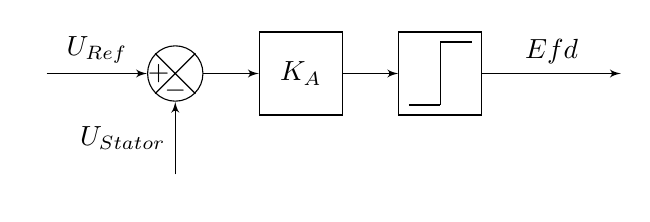
\begin{tikzpicture}
\sbEntree{E}
\sbCompSum[5]{errAVR}{E}{}{-}{+}{}
\sbRelier[$U_{Ref}$]{E}{errAVR}
\sbDecaleNoeudy[4]{errAVR}{Us}
\sbRelier[$U_{Stator}$]{Us}{errAVR}
\sbBloc{Gain}{$K_A$}{errAVR}
\sbRelier{errAVR}{Gain}
\sbBlocL{Limiter}{\tikz {\draw (-0.4,-0.4) -- (0,-0.4);\draw (0,-0.4) -- (0,0.4); \draw (0,0.4) -- (0.4,0.4); }}{Gain}
\sbSortie[5]{S}{Limiter}
\sbRelier[$Efd$]{Limiter}{S}
\end{tikzpicture}
\caption{Voltage regulator}
\end{figure}

For every machine the speed governor is as follows:
\begin{figure}[H]
\centering
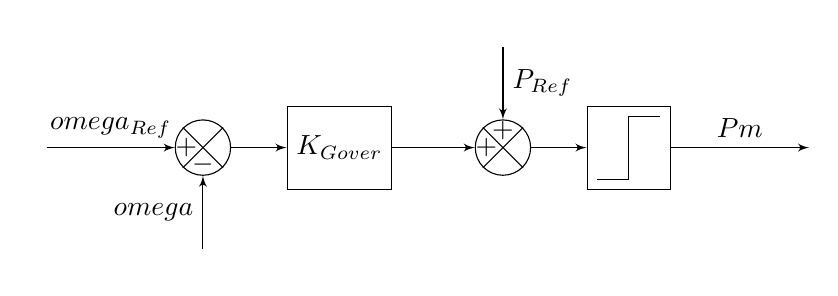
\begin{tikzpicture}
\sbEntree{E}
\sbCompSum[6]{errW}{E}{}{-}{+}{}
\sbRelier[$omega_{Ref}$]{E}{errW}
\sbDecaleNoeudy[4]{errW}{Omega}
\sbRelier[$omega$]{Omega}{errW}
\sbBloc{Gain}{$K_{Gover}$}{errW}
\sbRelier{errW}{Gain}
\sbCompSum{sumP}{Gain}{+}{}{+}{}
\sbRelier{Gain}{sumP}
\sbDecaleNoeudy[-4]{sumP}{PRef}
\sbRelier[$P_{Ref}$]{PRef}{sumP}
\sbBlocL{Limiter}{\tikz {\draw (-0.4,-0.4) -- (0,-0.4);\draw (0,-0.4) -- (0,0.4); \draw (0,0.4) -- (0.4,0.4); }}{sumP}
\sbSortie[5]{S}{Limiter}
\sbRelier[$Pm$]{Limiter}{S}
\end{tikzpicture}
\caption{Speed Governor}
\end{figure}

For every machine the voltage regulator parameters are:
\begin{center}
\begin{tabular}{l|l}
   $K_A=20$ & $Efd_{Max}=5$  \\
    & $Efd_{Min}=-5$   \\
\end{tabular}
\end{center}

For every machine the speed governor parameters are:
\begin{center}
\begin{tabular}{l|l}
   $P_{Nom}=S_{Nom_{SM}}$ & $P_{Max}=S_{Nom_{SM}}$  \\
   $K_{Gover}=5$ & $P_{Min}=0$   \\
\end{tabular}
\end{center}

All other parameters (physical behaviour, transformer, etc...) can be found in each scenario's IEEE14.par file.

\subsubsection{System reference frequency}

The system reference frequency used in every machine's model is computed as following:

\[
 \omega_{ref} = \sum_{Gen \hspace{2pt} n} H_{n} Snom_{n} \omega_{n}
\]

where $H_{n}$ is generator n inertia and $Snom_{n}$ its apparent power.
\subsubsection{Loads}

Loads follow an alpha beta dynamic behaviour, that is to say :

\[
\begin{aligned}
& P = P_{ref} (\frac{U}{U_{0}})^\alpha \\
& Q = Q_{ref} (\frac{U}{U_{0}})^\beta
\end{aligned}
\]
with $\alpha$ = 1.5 and $\beta$ = 2.5 \\
They are directly connected to the grid (no transformer included).


\subsection{Scenarios}
The simulated scenarios are :
\begin{itemize}
\item a disconnection of generator 2 [\ref{DisconnectGenerator}];
\item a disconnection of line 1-5 [\ref{DisconnectLine}];
\item a load variation on bus 2 [\ref{LoadVariation}];
\end{itemize}

\subsection{Solver}
The solver used is the variable time step solver IDA with the following parameters:
\begin{itemize}
\item $Order$=2;
\item $Accuracy_{Rel}$=10e-4;
\item $Accuracy_{Abs}$=10e-4;
\end{itemize}


\newpage
\section{Results}

For each event, we focus on generator 1 's response.

\subsection{Generator Disconnection}
\label{DisconnectGenerator}

At $t=1s$, generator 2 is disconnected.\\

As generator 2 was injecting active and reactive power, we observe that its loss entails both a voltage and a frequency drop for the nearby generator 1. In response, the voltage and speed regulations raise their outputs and therefore the injected active and reactive powers, having generator 1 's voltage and frequency stabilize at a lower value.\\

\begin{figure}[H]
\subfigure[Active power (MW)]
{%
  \begin{tikzpicture}
    \begin{axis}[height = 2in]
        \addplot[color=blue!50]
        table[x=time, y=GEN____1_SM_generator_PGen]
        {../IEEE14_DisconnectGroup/reference/outputs/curves/curves.csv};
    \end{axis}
  \end{tikzpicture}
}
\subfigure[Omega (pu)]
{%
  \begin{tikzpicture}
    \begin{axis}[height = 2in, yticklabel style={/pgf/number format/.cd,fixed zerofill,precision=3}]
        \addplot[color=blue!50]
        table[x=time, y=GEN____1_SM_generator_omegaPu]
        {../IEEE14_DisconnectGroup/reference/outputs/curves/curves.csv};
    \end{axis}
  \end{tikzpicture}
}
\caption{Generator 1 response to the disconnection}
\end{figure}

\begin{figure}[H]
\subfigure[Reactive power (Mvar)]
{%
  \begin{tikzpicture}
    \begin{axis}[height = 2in]
        \addplot[color=blue!50]
        table[x=time, y=GEN____1_SM_generator_QGen]
        {../IEEE14_DisconnectGroup/reference/outputs/curves/curves.csv};
    \end{axis}
  \end{tikzpicture}
}
\subfigure[Stator voltage (kV)]
{%
  \begin{tikzpicture}
    \begin{axis}[height = 2in]
        \addplot[color=blue!50]
        table[x=time, y expr=\thisrow{GEN____1_SM_generator_UStatorPu}*24]
        {../IEEE14_DisconnectGroup/reference/outputs/curves/curves.csv};
    \end{axis}
  \end{tikzpicture}
}
\subfigure[Network voltage (kV)]
{%
  \begin{tikzpicture}
    \begin{axis}[height = 2in]
        \addplot[color=blue!50]
        table[x=time, y expr=\thisrow{NETWORK__BUS____1_TN_Upu_value}*69]
        {../IEEE14_DisconnectGroup/reference/outputs/curves/curves.csv};
    \end{axis}
  \end{tikzpicture}
}
\caption{Generator 1 response to the disconnection}
\end{figure}

\newpage
\subsection{Line Opening}
\label{DisconnectLine}

At $t=1s$, the line between buses 1 and 5 is opened at its bus 5 's extremity. 75.6 W and 3.1 Mvar of active and reactive power are initially transiting on this line (from bus 1 to bus 5).\\

We observe that the system is oscillating after the event but stabilizes after a few seconds. Due to the topology modification, the terminal voltage rises and then stabilize under the control of the voltage regulator. Minor changes are also induced on the evolution of generator 1 's frequency and its active power.\\

\begin{figure}[H]
\subfigure[Active power (MW)]
{%
  \begin{tikzpicture}
    \begin{axis}[height = 2in]
        \addplot[color=blue!50]
        table[x=time, y=GEN____1_SM_generator_PGen]
        {../IEEE14_DisconnectLine/reference/outputs/curves/curves.csv};
    \end{axis}
  \end{tikzpicture}
}
\subfigure[Omega (pu)]
{%
  \begin{tikzpicture}
    \begin{axis}[height = 2in, yticklabel style={/pgf/number format/.cd,fixed zerofill,precision=3}]
        \addplot[color=blue!50]
        table[x=time, y=GEN____1_SM_generator_omegaPu]
        {../IEEE14_DisconnectLine/reference/outputs/curves/curves.csv};
    \end{axis}
  \end{tikzpicture}
}
\caption{Generator 1 response to the disconnection}
\end{figure}

\begin{figure}[H]
\subfigure[Reactive power (Mvar)]
{%
  \begin{tikzpicture}
    \begin{axis}[height = 2in]
        \addplot[color=blue!50]
        table[x=time, y=GEN____1_SM_generator_QGen]
        {../IEEE14_DisconnectLine/reference/outputs/curves/curves.csv};
    \end{axis}
  \end{tikzpicture}
}
\subfigure[Stator voltage (kV)]
{%
  \begin{tikzpicture}
    \begin{axis}[height = 2in]
        \addplot[color=blue!50]
        table[x=time, y expr=\thisrow{GEN____1_SM_generator_UStatorPu}*24]
        {../IEEE14_DisconnectLine/reference/outputs/curves/curves.csv};
    \end{axis}
  \end{tikzpicture}
}
\subfigure[Network voltage (kV)]
{%
  \begin{tikzpicture}
    \begin{axis}[height = 2in]
        \addplot[color=blue!50]
        table[x=time, y expr=\thisrow{NETWORK__BUS____1_TN_Upu_value}*69]
        {../IEEE14_DisconnectLine/reference/outputs/curves/curves.csv};
    \end{axis}
  \end{tikzpicture}
}
\caption{Generator 1 response to the disconnection}
\end{figure}

\newpage
\subsection{Load Variation}
\label{LoadVariation}

At $t=1s$, the active and reactive power set points for the load on node 2 are doubled. The load value on node 2 is initially multiplied by 2 at $t=1s$ as expected and slightly decreases in the next instants to stabilize at a lower value (due to the voltage-dependant model used). \\

We observe that the reactive load variation triggers a sudden voltage drop at bus 1, which is contained and stabilized by a rise of generator 1's reactive power induced by the voltage regulator. Similarly, as the load active power consumption increases, the generator's frequency plummets before finding a lower steady state quickly thanks to the speed regulator.\\

\begin{figure}[H]
\subfigure[Active load (MW)]
{%
  \begin{tikzpicture}
    \begin{axis}[height = 1.4
   in, xmax=40]
        \addplot[color=blue!50]
        table[x=time, y expr= \thisrow{_LOAD___2_EC_load_PPu}*100]
        {../IEEE14_LoadVariation/reference/outputs/curves/curves.csv};
    \end{axis}
  \end{tikzpicture}
}
\subfigure[Reactive load (Mvar)]
{%
  \begin{tikzpicture}
    \begin{axis}[height = 1.4in]
        \addplot[color=blue!50]
        table[x=time, y expr=\thisrow{_LOAD___2_EC_load_QPu}*100]
        {../IEEE14_LoadVariation/reference/outputs/curves/curves.csv};
    \end{axis}
  \end{tikzpicture}
}
\subfigure[Network voltage (kV)]
{%
  \begin{tikzpicture}
    \begin{axis}[height = 1.4in]
        \addplot[color=blue!50]
        table[x=time, y expr=\thisrow{NETWORK__BUS____2_TN_Upu_value}*69]
        {../IEEE14_LoadVariation/reference/outputs/curves/curves.csv};
    \end{axis}
  \end{tikzpicture}
}
\caption{Load variation and voltage evolution on node 2}
\end{figure}

\begin{figure}[H]
\subfigure[Active power (MW)]
{%
  \begin{tikzpicture}
    \begin{axis}[height = 1.5in]
        \addplot[color=blue!50]
        table[x=time, y=GEN____1_SM_generator_PGen]
        {../IEEE14_LoadVariation/reference/outputs/curves/curves.csv};
    \end{axis}
  \end{tikzpicture}
}
\subfigure[Omega (pu)]
{%
  \begin{tikzpicture}
    \begin{axis}[height = 1.5in, yticklabel style={/pgf/number format/.cd,fixed zerofill,precision=3}]
        \addplot[color=blue!50]
        table[x=time, y=GEN____1_SM_generator_omegaPu]
        {../IEEE14_LoadVariation/reference/outputs/curves/curves.csv};
    \end{axis}
  \end{tikzpicture}
}
\subfigure[Reactive power (Mvar)]
{%
  \begin{tikzpicture}
    \begin{axis}[height = 1.5in]
        \addplot[color=blue!50]
        table[x=time, y=GEN____1_SM_generator_QGen]
        {../IEEE14_LoadVariation/reference/outputs/curves/curves.csv};
    \end{axis}
  \end{tikzpicture}
}
\subfigure[Stator voltage (kV)]
{%
  \begin{tikzpicture}
    \begin{axis}[height = 1.5in]
        \addplot[color=blue!50]
        table[x=time, y expr=\thisrow{GEN____1_SM_generator_UStatorPu}*24]
        {../IEEE14_LoadVariation/reference/outputs/curves/curves.csv};
    \end{axis}
  \end{tikzpicture}
}
\caption{Generator 1 response to the load variation}
\end{figure}

\end{document}
